\section{Evaluation}


\begin{figure*}[tb]
    \centering
    \begin{subfigure}[b]{0.33\textwidth}
        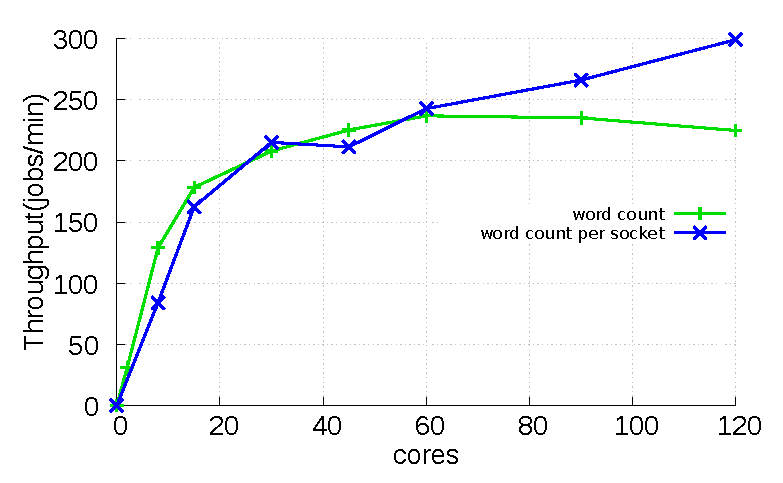
\includegraphics[width=2.2in]{graph/wc_docker.eps}
        \caption{Exim - 120core}
    \end{subfigure}%
    \begin{subfigure}[b]{0.33\textwidth}
        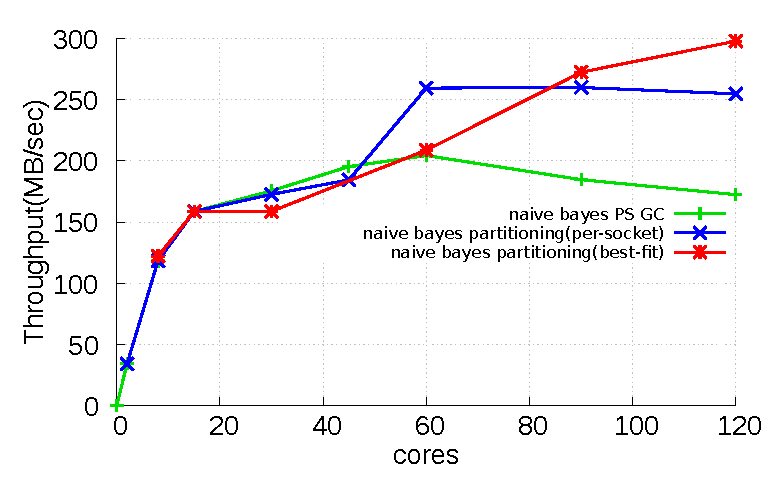
\includegraphics[width=2.2in]{graph/nb_docker.eps}
        \caption{Lmbench - 120core}
    \end{subfigure}%
    \begin{subfigure}[b]{0.33\textwidth}
        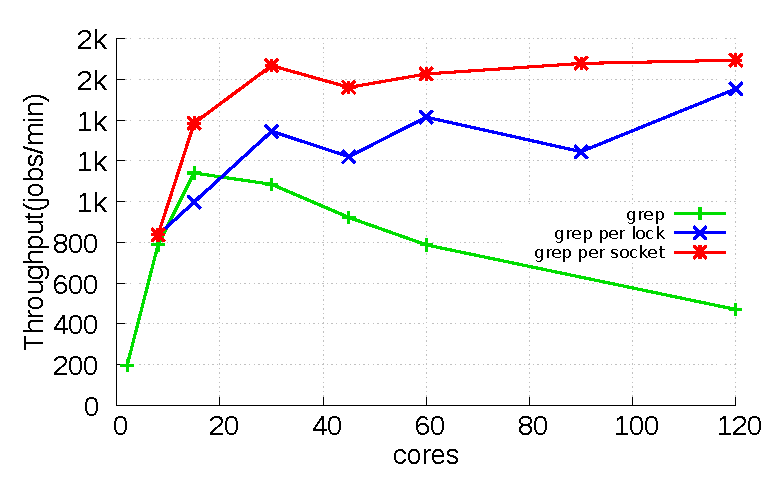
\includegraphics[width=2.2in]{graph/grep_docker.eps}
        \caption{AIM7 - 120core}
    \end{subfigure}
        \begin{subfigure}[b]{0.33\textwidth}
        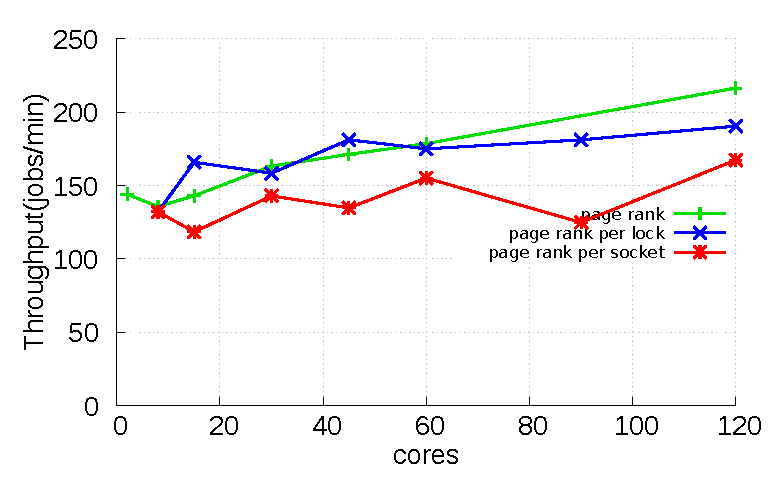
\includegraphics[width=2.2in]{graph/pagerank_docker.eps}
        \caption{Lmbench - 120core}
    \end{subfigure}%
        \begin{subfigure}[b]{0.33\textwidth}
        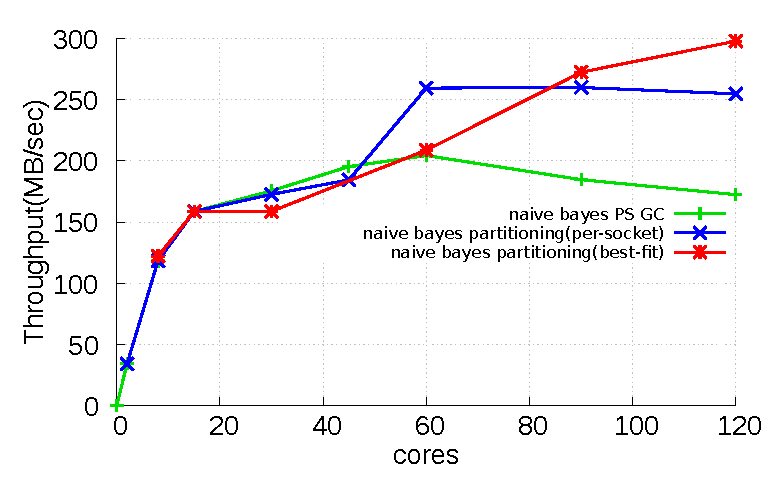
\includegraphics[width=2.2in]{graph/nb_docker.eps}
        \caption{Lmbench - 120core}
    \end{subfigure}%
        \centering
    \caption{CPU utilization on 120 core.}
    \label{fig:utilization3}
\end{figure*}





\begin{figure*}[tb]
    \centering
    \begin{subfigure}[b]{0.20\textwidth}
        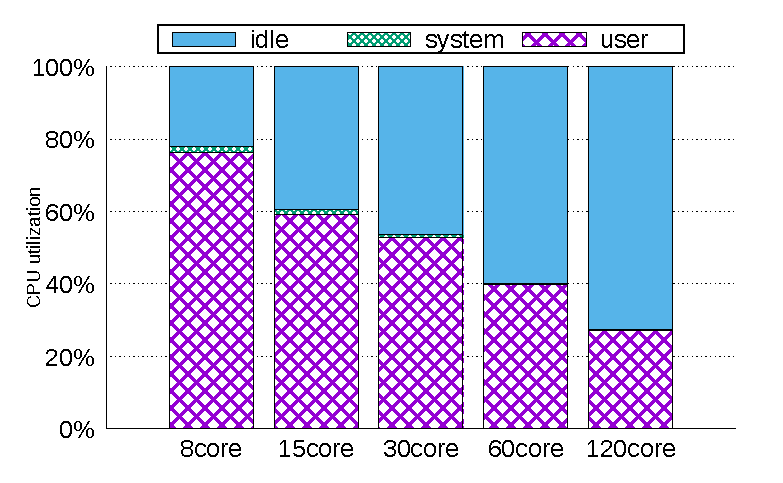
\includegraphics[width=1.4in]{graph/wc_cpuutils.eps}
        \caption{Word Count}
    \end{subfigure}%
    \begin{subfigure}[b]{0.20\textwidth}
        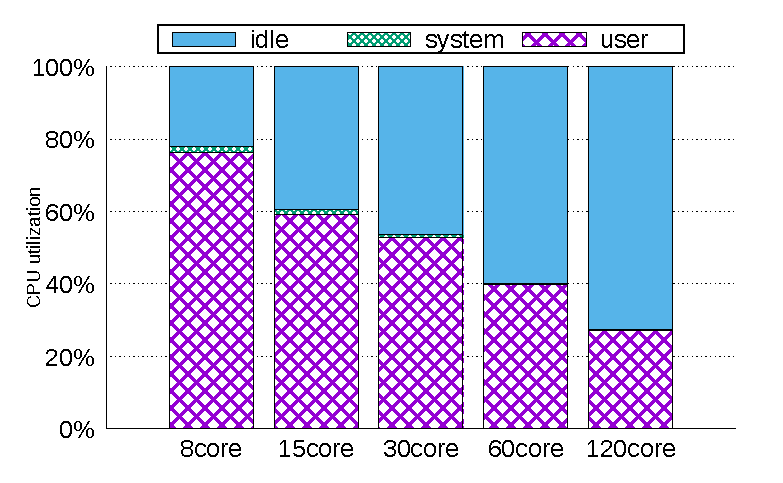
\includegraphics[width=1.4in]{graph/wc_cpuutils.eps}
        \caption{Naive Basian}
    \end{subfigure}%
    \begin{subfigure}[b]{0.20\textwidth}
        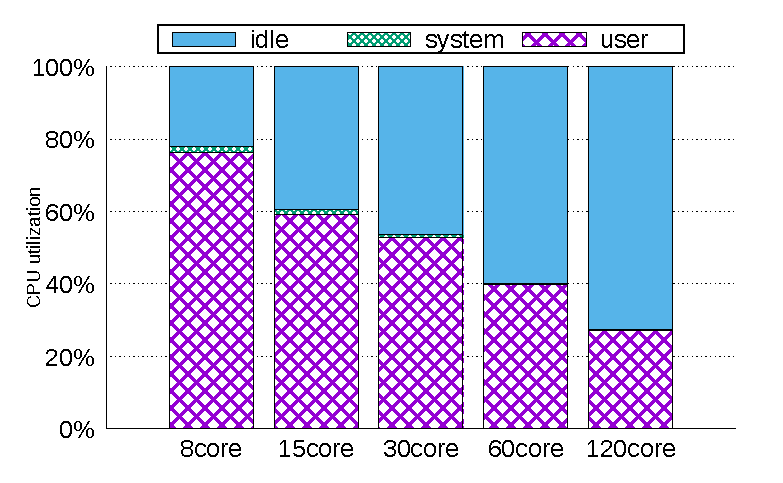
\includegraphics[width=1.4in]{graph/wc_cpuutils.eps}
        \caption{Grep}
    \end{subfigure}%
        \begin{subfigure}[b]{0.20\textwidth}
        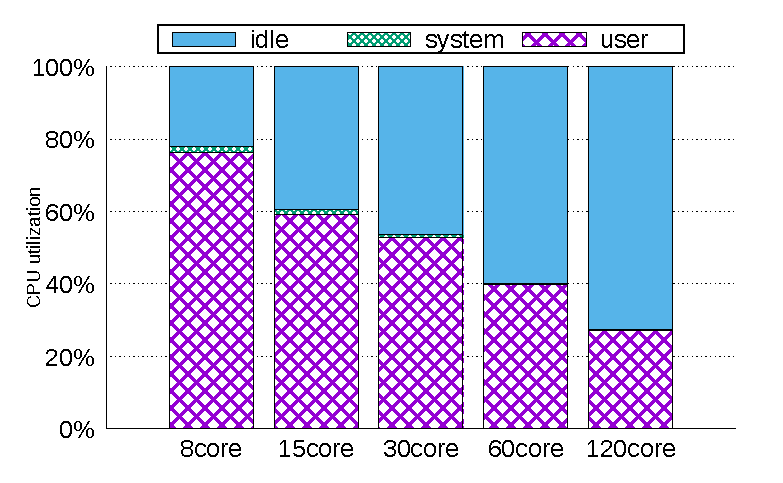
\includegraphics[width=1.4in]{graph/wc_cpuutils.eps}
        \caption{Pagerank}
    \end{subfigure}%
        \begin{subfigure}[b]{0.20\textwidth}
        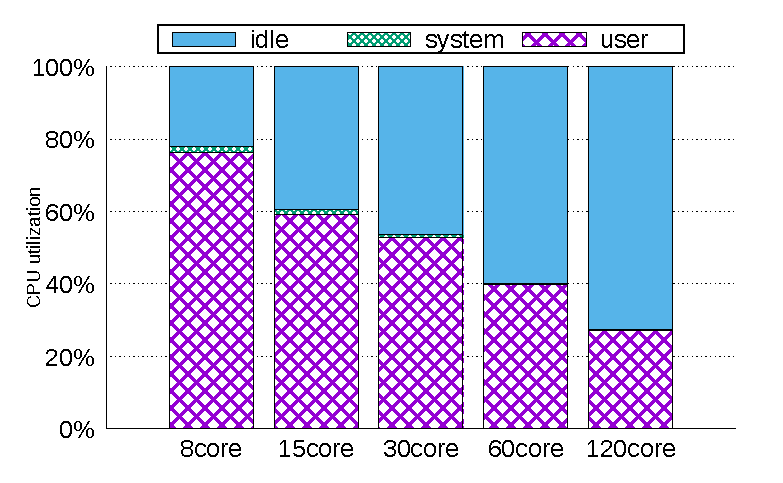
\includegraphics[width=1.4in]{graph/wc_cpuutils.eps}
        \caption{Pagerank}
    \end{subfigure}
        \centering
    \caption{CPU utilization on 120 core.}
    \label{fig:utilization2}
\end{figure*}


%$$$$$$$$$$$$$$$$$$$$$$$$$$$$$$$$$$$$$$$$$$$$$$$$$$$$$$$$$$$$$$$$$$$$$$$$$$$$$$$$
%Paragraph 1: 실험 환경 설명
%$$$$$$$$$$$$$$$$$$$$$$$$$$$$$$$$$$$$$$$$$$$$$$$$$$$$$$$$$$$$$$$$$$$$$$$$$$$$$$$$
\ifkor
이번 장에서는 스파크의 Scalalbility에 대해서 설명한다. 실험 환경은 2장에서 수행한 방법과
같은 플랫폼에서 실험을 하였고, 
We ran the three benchmarks on Linux 3.19.rc4 with stock Linux with 
the automatic NUMA balancing feature disabled because the
Harris linked list has the iteration issue~\cite{petrank2013lock}. 
All experiments were performed on a 120 core machine with 8-socket, 15-core
Intel E7-8870 chips equipped with 792 GB DDR3 DRAM.
\else

\fi




%$$$$$$$$$$$$$$$$$$$$$$$$$$$$$$$$$$$$$$$$$$$$$$$$$$$$$$$$$$$$$$$$$$$$$$$$$$$$$$$$
%Paragraph 2: 비교 대상 설명
%$$$$$$$$$$$$$$$$$$$$$$$$$$$$$$$$$$$$$$$$$$$$$$$$$$$$$$$$$$$$$$$$$$$$$$$$$$$$$$$$
\ifkor
이번 장에서는 스파크의 Scalalbility에 대해서 설명한다. 첫째로 
둘째로, NUMA socket 단위로 파티션닝을 수행한 방법이다. 우리의 시스템은 한 소켓당 15코어를
가지는 NUMA machine이므로 15개의 코어를 가지는 도커를 8개를 생성하여 동작시켰다.
Heap 메모리 설정은 표와 같다. 기본으로 4G의 메모리를 heap 메모리 사이즈로 설정하였고,
input 데이터는 10G 이상으로 설정하였다. 그 이유는 heap 메모리가 데이터 사이즈 보다 크면
scalabiliy가 문제가 없으나, 실제 1테라 이상의 데이터를 사용하는 big data
영역에서는 heap 메모리 사이즈가 데이터 사이즈보다 일반적으로 크기 때문이다.
그리고 메모리 설정은 파티션을 수행한 경우는 각 도커에 512MB로 설정하여 메모리 사용을 
동일하게 하여 동작 시켰다. 
\else

\fi


%$$$$$$$$$$$$$$$$$$$$$$$$$$$$$$$$$$$$$$$$$$$$$$$$$$$$$$$$$$$$$$$$$$$$$$$$$$$$$$$$
%Paragraph 2: default 설정 결과 설명 
%$$$$$$$$$$$$$$$$$$$$$$$$$$$$$$$$$$$$$$$$$$$$$$$$$$$$$$$$$$$$$$$$$$$$$$$$$$$$$$$$
\ifkor
그림 X-x는 실험 결과를 보여 준다. 대부분이 비슷한 양상을 보였고, 60코어 이하까지는
파티션한것과 Native와는 비슷한 결과를 가졌다. 하지만 60코어 이상이 되는 순간
도커 파티션닝 기법의 성능이 더 좋아지며, 120코어에서는 X배의 성능 항상을 이루었다.
그 이유는 파티션된 도커 워커에서 수행하는 것이 GC와 
NUMA의 영향과 operating system의 scalabilby 저해요소를 제거 했기 때문에 
Native로 수행한 것보다 높은 성능을 보였다. 
\else 

\fi


%$$$$$$$$$$$$$$$$$$$$$$$$$$$$$$$$$$$$$$$$$$$$$$$$$$$$$$$$$$$$$$$$$$$$$$$$$$$$$$$$
%Paragraph 2: 60코어 이후 결과 설명
%$$$$$$$$$$$$$$$$$$$$$$$$$$$$$$$$$$$$$$$$$$$$$$$$$$$$$$$$$$$$$$$$$$$$$$$$$$$$$$$$
\ifkor
AIM7 forks many processes, each of which concurrently runs. 
We used AIM7-multiuser, which is one of workload in AIM7.
The multiuser workload is composed of various workloads such as disk-file
operations, process creation, virtual memory operations, pipe I/O, and
arithmetic operation.
To minimize IO bottlenecks, the workload was executed with tmpfs filesystems, each
of which is 10 GB.
\else

\fi




%$$$$$$$$$$$$$$$$$$$$$$$$$$$$$$$$$$$$$$$$$$$$$$$$$$$$$$$$$$$$$$$$$$$$$$$$$$$$$$$$
%Paragraph 2: pagerank 결과에 대한 설명
%$$$$$$$$$$$$$$$$$$$$$$$$$$$$$$$$$$$$$$$$$$$$$$$$$$$$$$$$$$$$$$$$$$$$$$$$$$$$$$$$
\ifkor
AIM7 forks many processes, each of which concurrently runs. 
We used AIM7-multiuser, which is one of workload in AIM7.
The multiuser workload is composed of various workloads such as disk-file
operations, process creation, virtual memory operations, pipe I/O, and
\else

\fi



%$$$$$$$$$$$$$$$$$$$$$$$$$$$$$$$$$$$$$$$$$$$$$$$$$$$$$$$$$$$$$$$$$$$$$$$$$$$$$$$$
%Paragraph 2: CPU utilization에 대한 설명
%$$$$$$$$$$$$$$$$$$$$$$$$$$$$$$$$$$$$$$$$$$$$$$$$$$$$$$$$$$$$$$$$$$$$$$$$$$$$$$$$
\ifkor
AIM7 forks many processes, each of which concurrently runs. 
We used AIM7-multiuser, which is one of workload in AIM7.
The multiuser workload is composed of various workloads such as disk-file
operations, process creation, virtual memory operations, pipe I/O, and
\else

\fi
